\chapter{Project description}
This chapter thoroughly goes through the project describing each aspect with focus on what is important and what the group has learned through the project.
\section{Analysis}
This section describes the analysis which went ahead before implementing anything on the DSP. Most of the analysis is made in Matlab and/or mathcad. Therefore there will be some code and calculations from these programs.\\
In the analysis section we will conclude on our findings after each subsection
\subsection{Platform}
Before the project went ahead with anything we wanted to settle on a platform to implement our system. Below is an analysis of some platforms which were available.
\subsubsection{PSoC}
\textbf{Speed:}\\
The PSoC 3 system has a single core running up to 67 MHz. It does not have arithmetic calculation so it might not be ideal for large DSP operations such as cross correlation. \\
\textbf{I/O:}\\
The PSoC has 28 GPIO pins. These can be configured any way you want. The range of the pins is 1.7 V to 5.5 V depending on supply voltage. \\
\textbf{ADC/DMA:}\\
PSoC has a 24-channel DMA which is programmable to access nearly every bus on the board. It has both delta-sigma and sar ADC with up to 20 bits resolution. Sample rate can be up to 192 kHz at 12 bit resolution. \\
\textbf{Memory:}\\
The PSoC has 64 KB of flash memory, 8 KB SRAM and 512-byte cache. This would be enough memory for small signals but would prove difficult if we were to use larger audio signals.\\
\subsubsection{Blackfin}
\textbf{Speed:}\\
The blackfin processor runs at 600MHz. For every clock it can do two operations (multiplication and/or addition). This effectively means that we can do 1200 million operations per second, if we use the processor 100\% of the time.\\
\textbf{I/O:}\\
The blackfin has an output range of 0 - 0.4 V low to 2.4 - 3.6 high. Input range is -0.3 to 3.6 V. Most of the blackfins I/O is controller by ports. All the phono plugs are connected to the port "Sport0". 
\textbf{ADC \& Audiocodec:}\\
The blackfin has a built-in audiocodec consisting of 4 ADCs and 6 DACs with a resolution of 24 bits. It has a signal to noise ratio of 105dB\footnote{http://www.analog.com/en/audiovideo-products/audio-codecs/ad1836/products/product.html}. There is an example project in the VisualDSP++ environment explaining how to utilize this codec.\\
\textbf{Memory:}\\
Since we do not use much memory we use the L1 cache in the BF533. It is according to the datasheet 32Kbytes big. Since we work with the datatype "short", which is 16 bits, we have enough space for 16K samples.\\
\begin{figure}[hbpt]
\centering
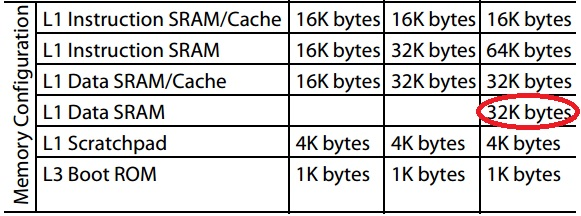
\includegraphics[width=0.5\textwidth]{billeder/memorytable}
\caption[Screen dump from datasheet]{Screen dump from datasheet\footnotemark}
\label{img:mem_table}
\end{figure}
\footnotetext{\url{http://www.analog.com/static/imported-files/data_sheets/ADSP-BF531_BF532_BF533.pdf}}
\subsubsection{DK8K}
We chose to ignore the DK8K platform as it does not have an Interactive Developer Environment(IDE). This would put a bigger workload on us but would not help us understand how to take advantage of Digital signal processing on embedded units.
%Johnny - Jeg synes ikke det her skal være med.
\subsection{Fixed-/floating point}
\subsubsection{Floating Point}
Floating point is a way of give approximation of a real value. Usually when working with floating point we have a fixed number of significant digits. A way of presenting a floating point number is "1.2345". Floating point types in c are double and float. The main advantage of floating point is high precision. This comes at a cost of performance and component price.
\subsubsection{Fixed Point}
Fixed point arithmetic is a way to represent a number that has a fixed number of digits before and after the the decimal "." point. Fixed point arithmetic is especially useful for representing fract data types in base 2 or base 10. A way to represent "1.23" in fixed point is "1230". A scaling factor was used. Scaling factors are usually base 2 or base 10. The main advantage of fixed point is performance. This comes at a price of precision. Some embedded microprocessors can not process floating point as it requires a floating point unit(FPU).\\

\subsection{Technology/equipment}
\subsubsection{Ultrasound}
The first method we discussed was ultrasound. But if we were to choose ultrasound we wouldnt have much data processing since we would just have a transmitter/reciever circuit which has an electrical interface. And wo wouldnt learn much about implementing digital signal processing.\\
\textbf{Equipment}\\
We had an ultrasonic distance sensor available, but it had a simple electrical interface and it wouldn't imply much signal processing since it would be mostly timing based.
\subsubsection{Laser}
We didnt realy consider laser since we would rather try to play around with sound and measurements of sound. We also figured it would be a lot more complicated for this type of project.
%%%%%%%%%%%%SKAL DET VÆRE HER??%%%%%%%%
\subsubsection{Audio}
We went along with hearable sound by suggestion from Peter. Hearable sound is easier to work with since, yes we can hear it, but it is easier to measure and produce. When we record sound we also get a lot of sample which we can process.\\
\textbf{Equipment}\\
We had both speaker and microphones available.
\subsection{Cross-correlation}
\subsubsection{Theory}
Cross-correlation is a method used for comparing two signals. This can for example be with the purpose of finding specific features, patterns or identical signals.


\begin{equation}
\label{eq:xcross}
\centering
(f\star g)(t)=\sum\limits_{m=-\infty}^{m=\infty}f(t)*g(t+m)
\end{equation}
The equation in \ref{eq:xcross} is the mathematical expression of cross-correlation of discrete functions.

In figure \ref{fig:xcrossSample} two signals are present. We can use cross-correlation to find out how much these two signals are similar. This can be done using equation \ref{eq:xcross}. Since our signal doesn't go to $\infty$, but only to 7, we will let $m=-7$ to $m=7$, so our equation will be the one shown in \ref{eq:xcross2}.

\begin{equation}
\label{eq:xcross2}
\centering
(f\star g)(t)=\sum\limits_{m=-7}^{m=7}f(t)*g(t+m)
\end{equation}

We can establish from the graph that the two signals have consist of the two following data sets:
Green: \[0,1,2,1,0,0,0\]
Blue: \[0,0,0,1,2,1,0\]
These are the data points from 1-7. Any data point outside of that range will be zero. We will also use $t=-7$ to $t=7$ to cover the negative side in case of a left side shift.

We can then, following equation \ref{eq:xcross2}, calculate the cross-correlation:

\begin{center}
$(f\star g)(-7)=f(-7)*g(-7+(-7)+f(-7)*g(1+(-6))+...+f(-7)*g(-7+6)+f(1)*g(-7+7)$\\
$(f\star g)(-6)=f(-6)*g(-6+(-7)+f(-6)*g(2+(-6))+...+f(-6)*g(-6+6)+f(2)*g(-6+7)$\\
$(f\star g)(-5)=f(-5)*g(-5+(-7)+f(-5)*g(3+(-6))+...+f(-5)*g(-5+6)+f(3)*g(-5+7)$\\
$(f\star g)(-4)=f(-4)*g(-4+(-7)+f(-4)*g(4+(-6))+...+f(-4)*g(-4+6)+f(4)*g(-4+7)$\\
$(f\star g)(-3)=f(-3)*g(-3+(-7)+f(-3)*g(5+(-6))+...+f(-3)*g(-3+6)+f(5)*g(-3+7)$\\
$(f\star g)(-2)=f(-2)*g(-2+(-7)+f(-2)*g(6+(-6))+...+f(-2)*g(-2+6)+f(6)*g(-2+7)$\\
$(f\star g)(-1)=f(-1)*g(-1+(-7)+f(-1)*g(7+(-6))+...+f(-1)*g(-1+6)+f(7)*g(-1+7)$\\
$(f\star g)(0)=f(0)*g(0+(-7)+f(0)*g(0+(-6))+...+f(0)*g(0+6)+f(0)*g(0+7)$\\
$(f\star g)(1)=f(1)*g(1+(-7)+f(1)*g(1+(-6))+...+f(1)*g(1+6)+f(1)*g(1+7)$\\
$(f\star g)(2)=f(2)*g(2+(-7)+f(2)*g(2+(-6))+...+f(2)*g(2+6)+f(2)*g(2+7)$\\
$(f\star g)(3)=f(3)*g(3+(-7)+f(3)*g(3+(-6))+...+f(3)*g(3+6)+f(3)*g(3+7)$\\
$(f\star g)(4)=f(4)*g(4+(-7)+f(4)*g(4+(-6))+...+f(4)*g(4+6)+f(4)*g(4+7)$\\
$(f\star g)(5)=f(5)*g(5+(-7)+f(5)*g(5+(-6))+...+f(5)*g(1+6)+f(5)*g(5+7)$\\
$(f\star g)(6)=f(6)*g(6+(-7)+f(6)*g(6+(-6))+...+f(6)*g(2+6)+f(6)*g(6+7)$\\
$(f\star g)(7)=f(7)*g(7+(-7)+f(7)*g(7+(-6))+...+f(7)*g(3+6)+f(7)*g(7+7)$\\
\ \\
$(f\star g)(1)=$\\
$(f\star g)(2)=$\\
$(f\star g)(3)=$\\
$(f\star g)(4)=$\\
$(f\star g)(5)=$\\
$(f\star g)(6)=$\\
$(f\star g)(7)=$\\
\end{center}

Instead of letting m be in the range of $-\infty$ to $\infty$, we will let our sample size control the range, as in equation \ref{eq:xcrossN}
\begin{equation}
\label{eq:xcrossN}
\centering
(f\star g)(t)=\sum\limits_{m=-N}^{m=N}f(t)*g(t+m)
\end{equation}

\subsubsection{Signal analysis}
Before we went any further with the project we investigated which kind of signals which was good to send. We did that by generating a signal, made a delay and then cross-correlated these two signals, chirp, sinusoid and noise.
We tried three different signals\\
\textbf{Chirp}:\\
We started with a chirp. We did that because of gut feeling. We thought this would be the best signal to send mostly because it was controlled and not random, and the signal changed characteristic over time.\\
Below is shown the code we used to generate the signal, make the delay and do the cross-correlation:
\begin{lstlisting}[language=Matlab,frame=lrtb,label=Matlab Code for Chirp Cross-correlation]
Fs=48000;                                       % Sample frequency
t = [0:1/Fs:1];                                % Timeinterval and length
Frq1=14000;                                     % Start frequency for chirp
Frq2=14100;                                     % End frequency for chirp
delay = 2000;                                   % Signal Delay
Chirp_signal=chirp(t,Frq1,1,Frq2);              % Chirp signal generation
Chirp_delayed=[zeros(1,delay) Chirp_signal];    % Chip delay generation
Chirp_xcorr=xcorr(Chirp_signal,Chirp_delayed);  % Cross-correlation
LengthChirp_xcorr=length(Chirp_xcorr)           % Calculate length of Xcorr
[XmaxChirp_xcorr,YmaxChirp_xcorr]=max(Chirp_xcorr) % Find maximum value
Delay_calcX1X2=((LengthChirp_xcorr+1)/2)-YmaxChirp_xcorr % Calculate Delay
\end{lstlisting}
Below is the plot of the cross-correlation. It shows clearly where the to signal overlap.\\
\begin{figure}[H]
\centering
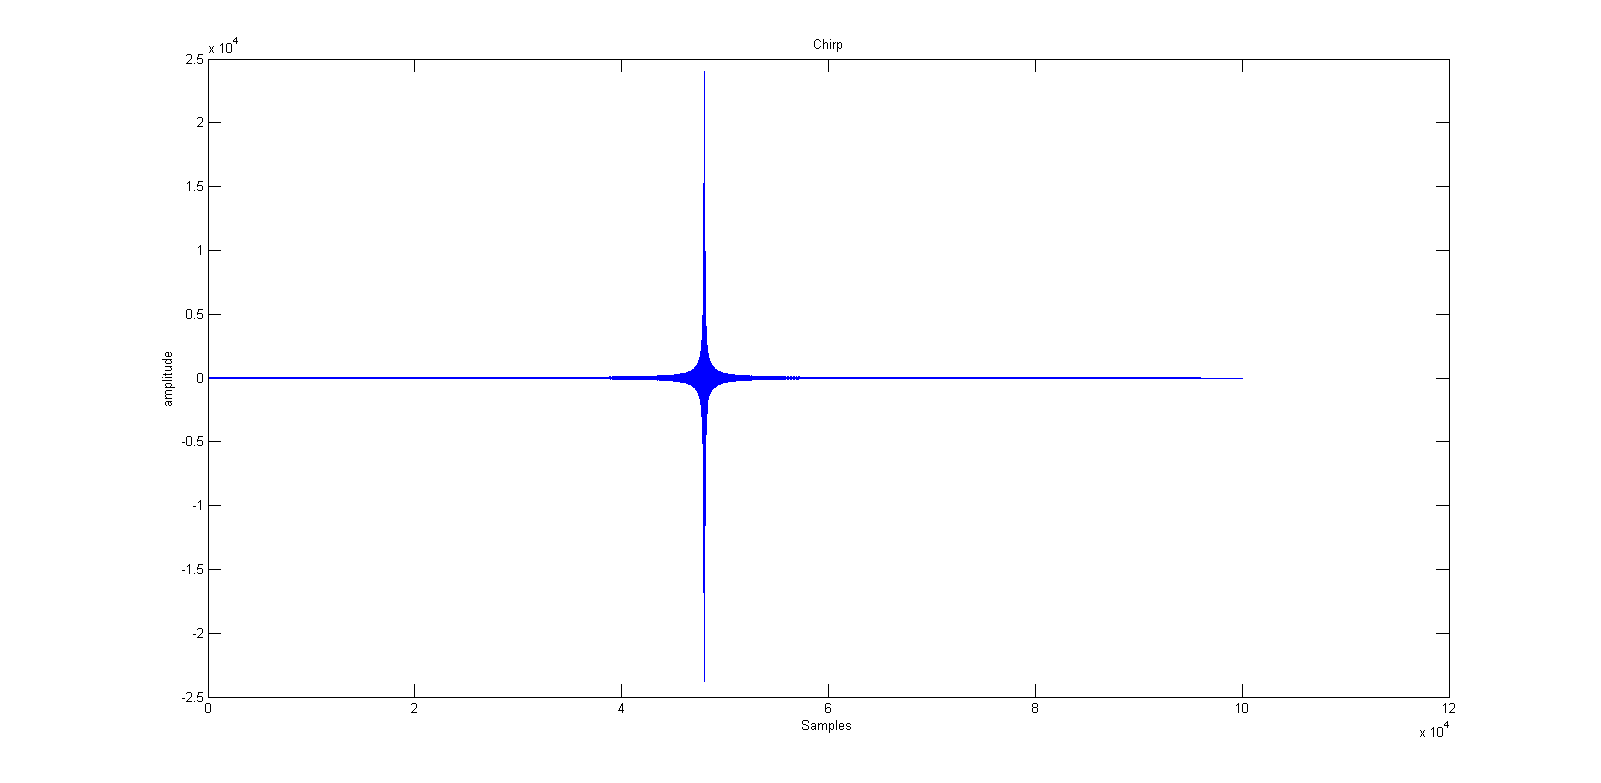
\includegraphics[width=0.6\textwidth]{billeder/chirp_xcorr_fig}
\caption{Plot of Cross-correlation of chirp signals}
\label{fig:chirp_xcorr_plot}
\end{figure}
The figure clearly shows where the two signals perfectly overlap. So the chirp seems like a good signal to use. although it isn't perfectly sharp in one sample it is quite distinct.\\
\textbf{Sinusoid}:\\
Similar code as the chirp was used to make two sinusoid signal. Below is a plot of a 14kHz sinus delayed with the same amount as the chrip signal.\\
\begin{figure}[H]
\centering
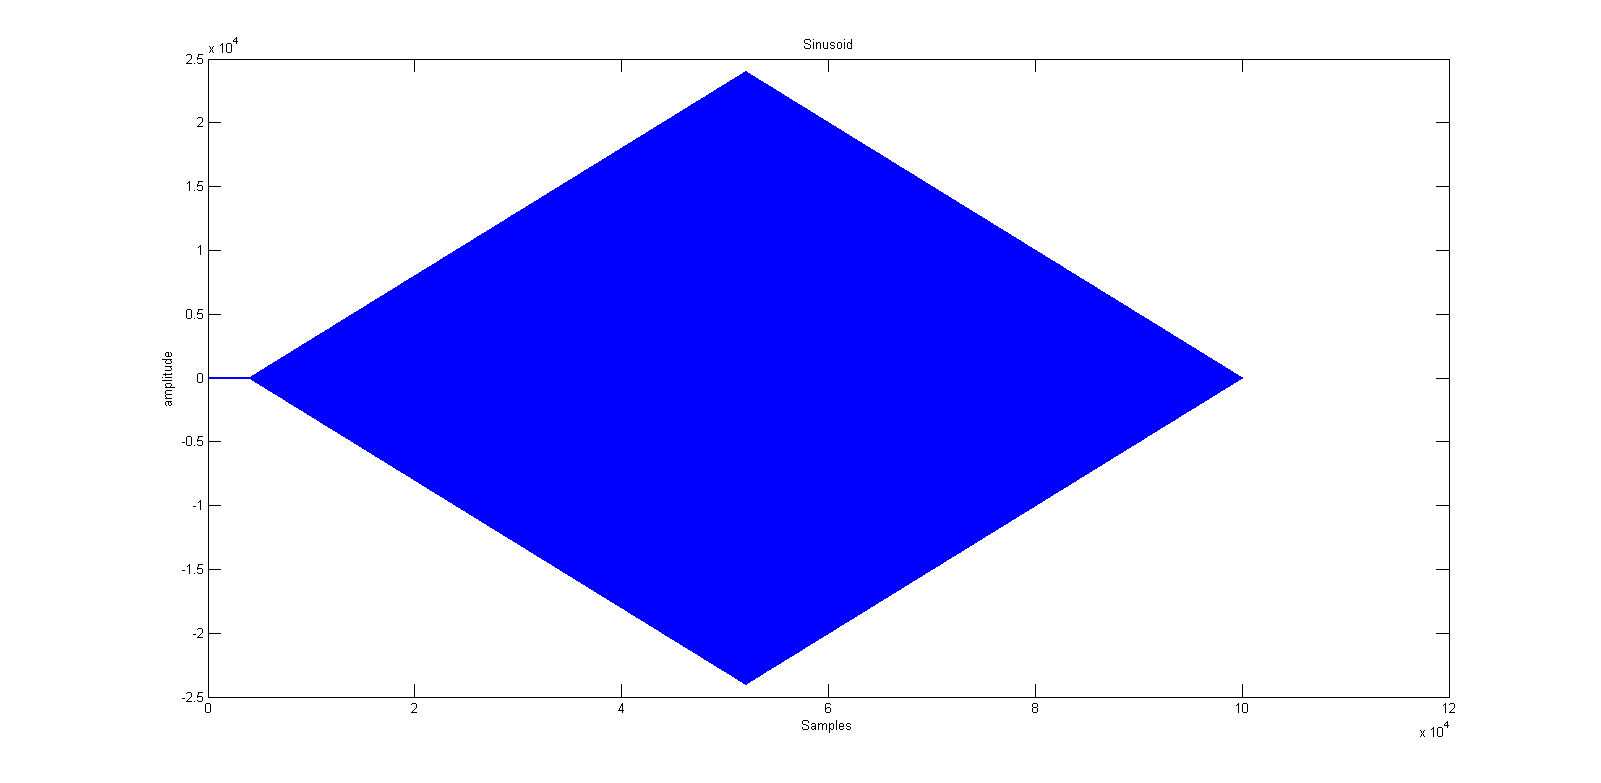
\includegraphics[width=0.6\textwidth]{billeder/sinus_xcorr_fig}
\caption{Plot of Cross-correlation of sinusoid signal}
\label{fig:sinus_xcorr_plot}
\end{figure}
This cross-correlation doesnt have as nice a peak as the chirp did and therefore we discarded using a sinusoid. The correlation looks like this because the sinus will make a spike every period because the periods will overlay eachother, this will increase until the signals completely overlays eachother.\\
\textbf{Noise}:\\
Lastly we tried generating a noise signal using the built-in function wgn (white gaussian noise). Below is shown the cross-correlation of the noise signals.\\
\begin{figure}[H]
\centering
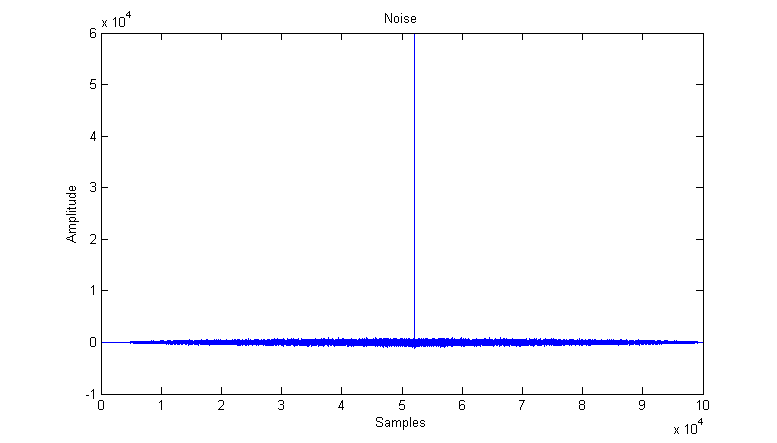
\includegraphics[width=0.6\textwidth]{billeder/noise_xcorr_fig}
\caption{Plot of cross-correlation of noise signal}
\label{fig:noise_xcorr_plot}
\end{figure}
This correlation made an even harder spike then the chirp. This is because of the fact that the  two noise signal only are similar in a very specific point. When they are not completely overlaying each other most samples end up cancelling each others.
\subsection{Findings based on examination in matlab}
It is clear that the chirp as well as the noise are very distinct peaks where the signals overlap. 

\subsubsection{Distance and signal}
%Måske noget med hvor store vores buffere skal være og hvor "lang" lyden er i aftand i forhold til samples osv? måske i stedet under implemenation
\subsection{Output}
\textbf{UART}:\\
VisualDSP++ comes with an example project for UART. We tried running the example project but we had no luck. We could not get the example project to work. We searched the internet for other example projects but still, we could not get them to work. \\
\textbf{Sound}:\\
The original scope of our project was to have an audio source as our output, while using a sound to measure distance. This worked well since we already had the knowledge from the talkthrough on how to output sound.\\
We have a multitude of ways to create the sound we are playing. We could either create a sound in matlab and load it or we could create it directly on the blackfin. For testing purposes we chose the matlab solution. This would mean that once we have made the soundbits we wanted to use, we would have to convert them to a format known by the blackfin.
\subsection{Convert to BF}
The blackfin has a small "hack" when it comes to loading sound from memory:
\begin{lstlisting}[language=C]
short sound_buffer[length_of_signal] = { 
#include "signal_you_want_to_use.hex"
};
\end{lstlisting}
This means we have to convert our sound array to a hex format. The first thing we do when converting is reducing the amplitude of the signal to make sure it fits in a "c style short" datatype. Then we use a function "mydec2hex" which is an improved version of matlabs built-in function "dec2hex". After converting to hex-format we use the file descriptor to save the data into a hex file. The hex file is put in the project folder in VisualDSP++ and the codehack is put where you initialize your variables.
\subsection{VisualDSP++}
\subsubsection{Plot}
VisualDSP++ has a built-in function to plot data from the memory of the blackfin. This feature can be used when the blackfin has been flashed and then subsequently halted. To access this feature go into:
\begin{verbatim}
View -> Debug Windows -> Plot -> New
\end{verbatim}
Set name, length and type of the data you want to plot and press \"Add\". This way you can have multiple plots on the same graph. It is also possible to have multiple plots and to save the setting of your plot. An example of plot can be seen on figure~\ref{fig:visualdspplot}.
\begin{figure}[H]
\centering
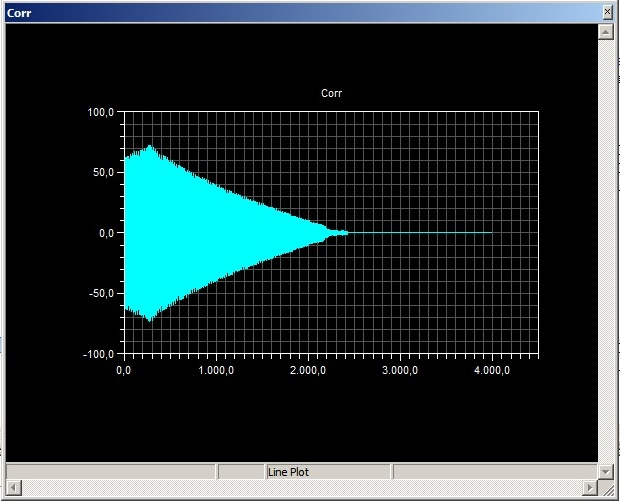
\includegraphics[scale=0.5]{billeder/visualdspplot}
\caption{Plot in VisualDSP++}
\label{fig:visualdspplot}
\end{figure}
\subsubsection{Memory dump}
A useful feature in VisualDSP++ is Memory dump. We can save the contents of arrays and variables directly onto the computer running VisualDSP++ in ".dat" format. To access this feature go into:
\begin{verbatim}
Memory -> Dump
\end{verbatim}
Set filename, type, size and variable/array name. Matlab can import these files directly. This feature is very useful when running tests and want to save data for later use or analysis.\\
\section{System architecture}
%Her skal vi lige finde ud af hvad vi skal have og om vi skal have det??

\section{Design and implementation}

\subsection{Considerations}
\subsubsection{Built-in functions}
\subsubsection{Output}
\subsubsection{Buffer sizes}

\section{Blackfin Setup}

\section{Important code description}

\section{Our Cross-correlation implementation}


\section{Tests and results}
\subsection{Total System}
\subsubsection{Test Setup}
\subsubsection{Test procedure}
\subsubsection{Test results}

\subsection{Test our cross-correlation}

\subsection{Compare our/built-in cross-correlation}


\section{Optimization}


\section{Obtained experience}